\begin{figure}[h!]
    \centering
    \caption{Minimum wage levels in the US by jurisdiction, 2010--2019}
    \label{fig:mw_policies}

    \begin{subfigure}{.7\textwidth}
        \caption{State policies}
        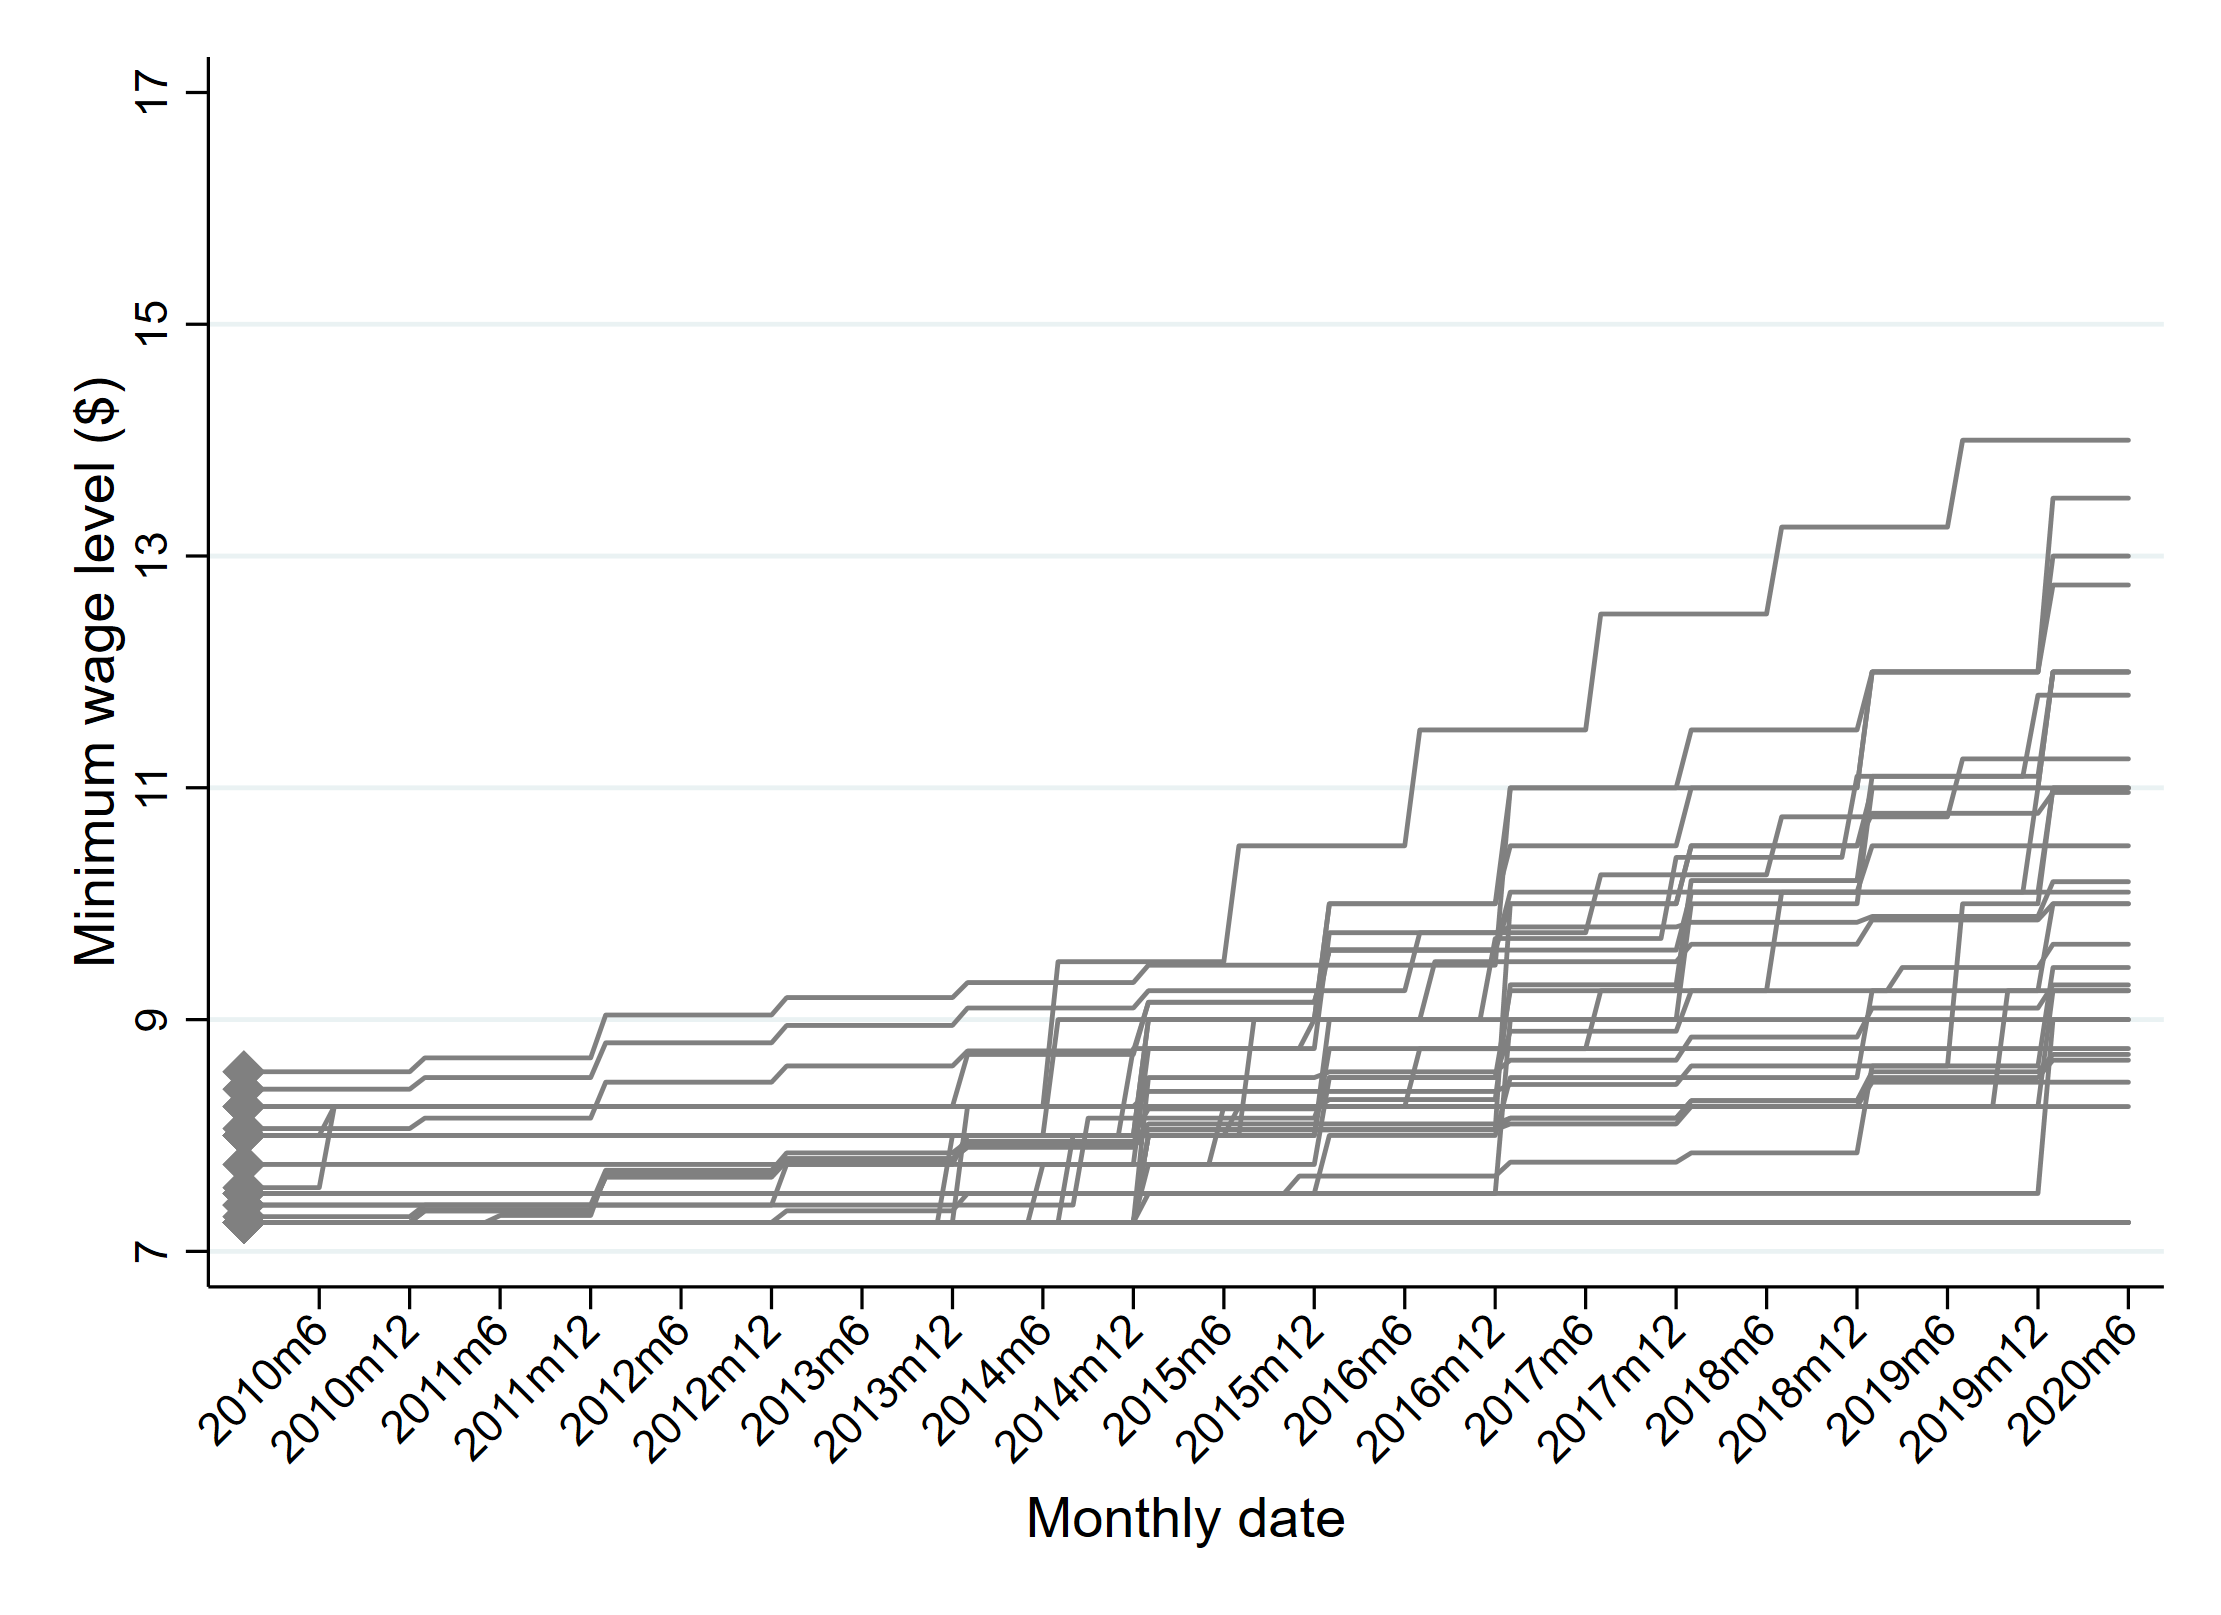
\includegraphics[width = \textwidth]
            {mw_US/output/state_mw_levels}
    \end{subfigure}\\
    \begin{subfigure}{.7\textwidth}
        \caption{Sub-state policies}
        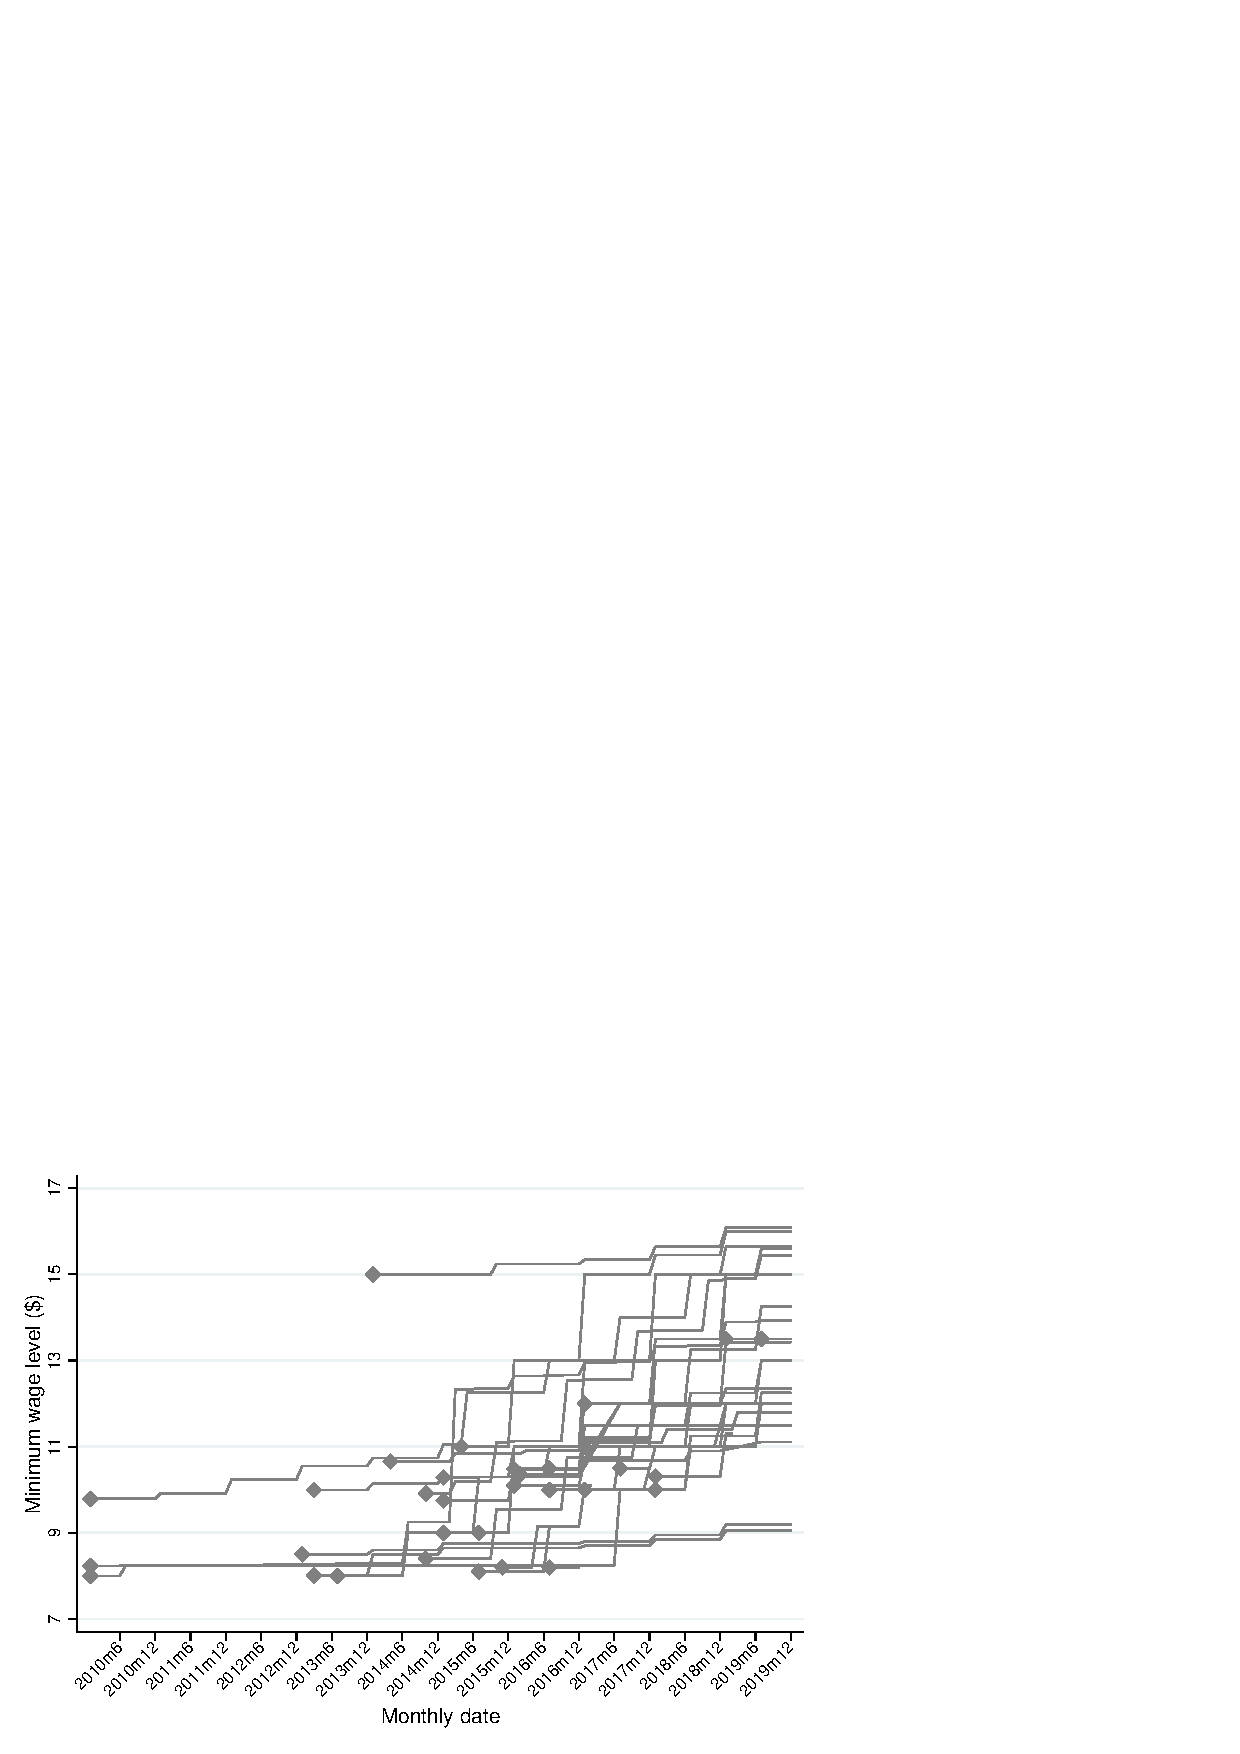
\includegraphics[width = \textwidth]
            {mw_US/output/local_mw_levels}
    \end{subfigure}

    \begin{minipage}{.95\textwidth} \footnotesize
        \vspace{3mm}
        Notes:
        Data are from the minimum wage panel described in 
        Section \ref{sec:data_mw_panel}.
        The lines in the plots show the levels of the minimum wage policies for 
        different jurisdictions that from January 2010 to December 2019 implemented 
        or changed such policy at least once between that period. 
        Diamonds indicate the first monthly date of a minimum wage policy 
        in the given jurisdiction.
        Panel (a) reports the state level policies.
        Panel (b) reports the sub-state level policies.
    \end{minipage}
\end{figure}
